\documentclass{article}
\usepackage[top=0.5in, bottom=0.5in, left=1.25in, right=1.25in]{geometry}

\usepackage{amsmath, array, enumerate, tikz, bm, pgfplots, pgfplotstable, tcolorbox, graphicx, venndiagram, color, colortbl}
\pgfplotsset{compat = newest}
\usepgfplotslibrary{statistics}
\renewcommand{\familydefault}{\sfdefault}
\raggedright
\pagestyle{empty}

\newcounter{example}[section]
\newenvironment{example}[1][]{\refstepcounter{example}\par\medskip
   {\color{red}\textbf{Example~\theexample. #1}}}{\medskip}

\begin{document}

\section*{Histograms}

\begin{tcolorbox}[colframe=orange!70!white, coltitle=black, title=\textbf{Summary}]
\begin{enumerate}
    \item Histograms are one of the most common visual displays of quantitative data.
    \item They can show frequencies, relative frequencies, or densities.
    \item Cumulative histograms display running totals.
\end{enumerate}
\end{tcolorbox}
\vspace{0.75in}

A {\color{blue}\textbf{histogram}} is like a bar graph but without any gaps between consecutive bars.

\begin{center}
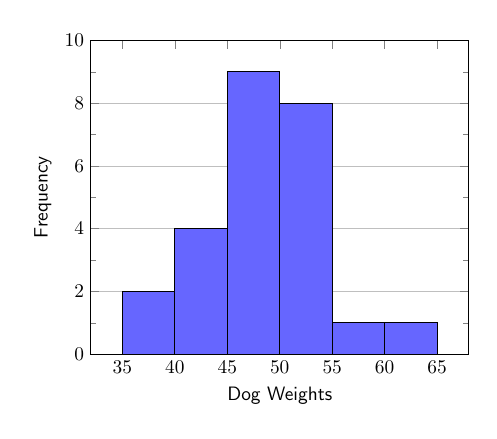
\begin{tikzpicture}[scale=0.7]
\begin{axis}[
ymin = 0, ymax = 10, xlabel = {Dog Weights}, ylabel = {Frequency}, ymajorgrids, minor y tick num = 1
]
\addplot[ybar interval, fill=blue!60, mark=no] plot coordinates {(35,2) (40,4) (45,9) (50,8) (55,1) (60,1) (65,1)};
\end{axis}
\end{tikzpicture}
\end{center}

\begin{itemize}
    \item Each bar is called a {\color{blue}\textbf{class}} (or {\color{blue}\textbf{bin}})
    \item The {\color{violet}\textbf{lower class limit}} of the first class is 35, of the 2nd class is 40, etc.
    \item The {\color{red}\textbf{class width}} in the above histogram is 5
    \item Each observed quantitative value is placed into a class or bin.
\end{itemize}

\vfill 

\begin{minipage}{0.35\textwidth}
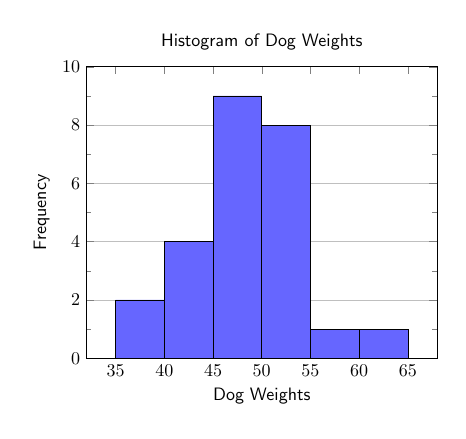
\begin{tikzpicture}[scale=0.65]
\begin{axis}[
ymin = 0, ymax = 10, xlabel = {Dog Weights}, ylabel = {Frequency}, ymajorgrids, minor y tick num = 1, title=Histogram of Dog Weights
]
\addplot[ybar interval, fill=blue!60, mark=no] plot coordinates {(35,2) (40,4) (45,9) (50,8) (55,1) (60,1) (65,1)};
\end{axis}
\end{tikzpicture}
\end{minipage}
\hspace{5pt}
\begin{minipage}{0.55\textwidth}
\scalebox{0.9}{
\begin{tabular}{c|c|c}
\textbf{Class} & \textbf{Frequency} & \textbf{Class Midpoint} \\ \hline
$35 \leq x < 40$ & 2 & 37.5 \\
$40 \leq x < 45$ & 4 & 42.5 \\
$45 \leq x < 50$ & 9 & 47.5 \\
$50 \leq x < 55$ & 8 & 52.5 \\
$55 \leq x < 60$ & 1 & 57.5 \\
$60 \leq x < 65$ & 1 & 62.5 
\end{tabular}}
\end{minipage}

\begin{center} 
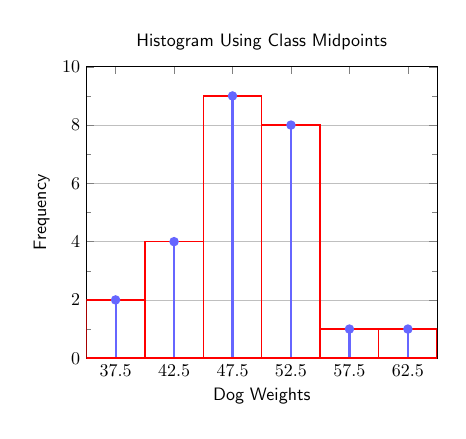
\begin{tikzpicture}[scale=0.65]
\begin{axis}[
xmin = 35, xmax = 65, xtick = {37.5,42.5,...,62.5}, ymin = 0, ymax = 10, xlabel = {Dog Weights}, ylabel = {Frequency}, ymajorgrids, minor y tick num = 1, title=Histogram Using Class Midpoints
]
\addplot[ycomb,color=blue!60,solid,mark=*, very thick] plot coordinates{ 
(37.5,2) (42.5,4) (47.5,9) (52.5,8) (57.5,1) (62.5,1)
};
\addplot+[ybar interval, mark=no, thick] plot coordinates {(35,2) (40,4) (45,9) (50,8) (55,1) (60,1) (65,1)};
\end{axis}
\end{tikzpicture}
\end{center}

\vfill 
\newpage 

\subsection*{Relative Frequency Histogram}

\begin{itemize}
    \item Create a relative frequency histogram much the same way we created relative frequency bar graphs.
    \item Total \emph{heights} of all rectangles must equal 1.00, or 100\%
\end{itemize}

\begin{center}
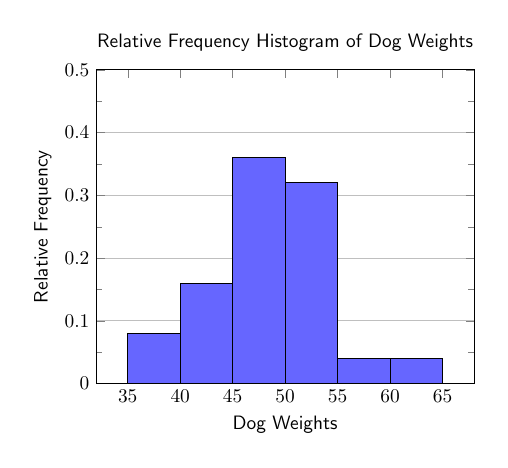
\begin{tikzpicture}[scale=0.7]
\begin{axis}[
ymin = 0, ymax = 0.5, xlabel = {Dog Weights}, ylabel = {Relative Frequency}, ymajorgrids, minor y tick num = 1, title=Relative Frequency Histogram of Dog Weights
]
\addplot[ybar interval, fill=blue!60, mark=no] plot coordinates {(35,2/25) (40,4/25) (45,9/25) (50,8/25) (55,1/25) (60,1/25) (65,1/25)};
\end{axis}
\end{tikzpicture}
\end{center}

\subsection*{Density Histogram}
\begin{itemize}
    \item Similar to a relative frequency histogram but the total {\color{red}\textbf{area}} of all rectangles must equal 1.
    \item We will see these \emph{a lot} with probability distributions later.
\end{itemize}

\begin{center}
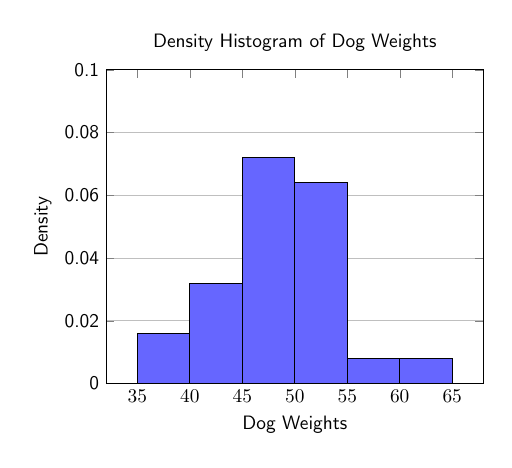
\begin{tikzpicture}[scale=0.7]
\begin{axis}[
ymin = 0, ymax = 0.1, 
xlabel = {Dog Weights}, 
ylabel = {Density}, 
yticklabels ={-0.02,0,0.02,0.04,0.06,0.08,0.1}, ymajorgrids, 
title=Density Histogram of Dog Weights
]
\addplot[ybar interval, fill=blue!60, mark=no] plot coordinates {(35,2/125) (40,4/125) (45,9/125) (50,8/125) (55,1/125) (60,1/125) (65,1/125)};
\end{axis}
\end{tikzpicture}
\end{center}

\vfill 

\begin{example}
Answer each of the following given the histogram below.  \newline\\
\begin{minipage}{0.45\textwidth}
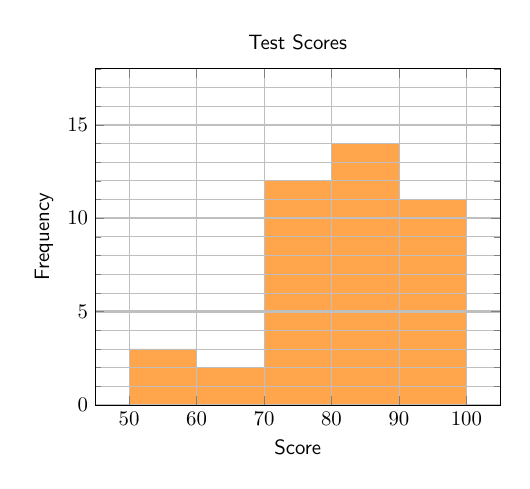
\begin{tikzpicture}[scale=0.75]
\begin{axis}[
    ymin=0, ymax=18, xlabel = {Score}, ylabel = {Frequency},
    minor y tick num = 4,
    area style, grid=both, major y grid style = {very thick},
    title=Test Scores
    ]
\addplot[ybar interval,mark=no, fill=orange!70, draw=black] plot coordinates { (50, 3) (60, 2) (70, 12) (80, 14) (90, 11) (100, 9)};
\end{axis}
\end{tikzpicture}
\end{minipage}
\begin{minipage}{0.3\textwidth}
\begin{enumerate}[(a)]  \setlength{\itemsep}{1.5cm}
    \item What is the class width?  
    \item What is the midpoint of the 4th class?
    \item What is the relative frequency of the 5th class?
\end{enumerate}
\end{minipage}
\end{example}

\vfill 
\newpage

\begin{example}
Create a histogram from the measurements below. Use the minimum value as the lower class limit of the first class and use a class width of 2.	\newline\\
\begin{tabular}{ccccc}
9& 2& 10& 1& 4	\\
5& 1& 6& 7& 4	\\
6& 5& 4& 8& 10	\\ 
3& 1& 2& 3& 9	\\
8& 6& 1& 1& 10
\end{tabular}
\end{example}
\vspace{2.5in}

\begin{example}
Use the histogram below of the weights of 200 dogs to answer each.    \newline\\

\begin{minipage}{0.45\textwidth}
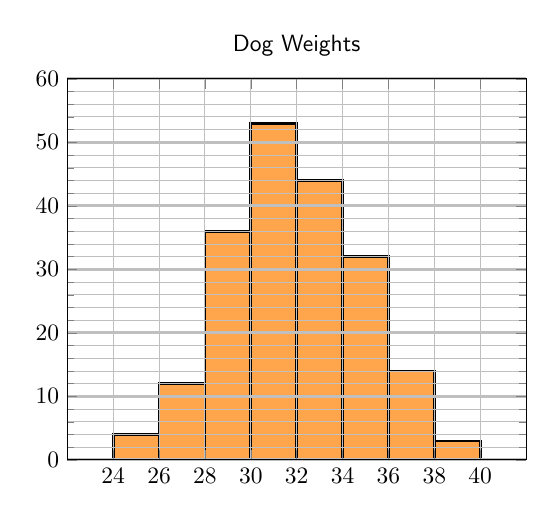
\begin{tikzpicture}[scale=0.85]
\begin{axis}[
    xmin = 22, xmax = 42, xtick = {24,26,...,40},
    ymin=0, ymax=60, ytick = {0,10,...,60},
    minor y tick num = 4,
    area style, major y grid style = {very thick}, grid=both, 
    title=Dog Weights
    ]
\addplot[ybar interval,draw=black, line width = 0.4mm, fill=orange!70] plot coordinates {
(24,4) (26,12) (28,36) (30,53) (32,44) (34,32) (36,14) (38,3) (40,3)
};
\end{axis}
\end{tikzpicture}
\end{minipage}
\begin{minipage}{0.35\textwidth}
\begin{enumerate}[(a)]  \setlength{\itemsep}{1.5cm}
    \item Find the total number of dogs whose weight is at least 34 pounds.
    \item What percentage of dogs have weights between 26 and 28 pounds?
\end{enumerate}
\end{minipage}
\end{example}

\vfill 
\newpage 

\subsection*{Cumulative Histograms}

A {\color{blue}\textbf{cumulative histogram}} is one in which the frequency (or relative frequency) of each class is a running total up to that class.
\vspace{0.75in}

\begin{example}
Use the table below to create a cumulative frequency histogram of dog weights from the beginning of the section.  \newline\\
\begin{tabular}{c|c|c}
\textbf{Class} & \textbf{Frequency} & \textbf{Total} \\ \hline
$35 \leq x < 40$ & 2 &  \\[6pt]
$40 \leq x < 45$ & 4 &  \\[6pt]
$45 \leq x < 50$ & 9 &  \\[6pt]
$50 \leq x < 55$ & 8 &  \\[6pt]
$55 \leq x < 60$ & 1 &  \\[6pt]
$60 \leq x < 65$ & 1 &  
\end{tabular}
\end{example}

\end{document}
